% -*- latex -*-
%-----------------------------------------------------------------------
%;  Copyright (C) 2005
%;  Associated Universities, Inc. Washington DC, USA.
%;
%;  This program is free software; you can redistribute it and/or
%;  modify it under the terms of the GNU General Public License as
%;  published by the Free Software Foundation; either version 2 of
%;  the License, or (at your option) any later version.
%;
%;  This program is distributed in the hope that it will be useful,
%;  but WITHOUT ANY WARRANTY; without even the implied warranty of
%;  MERCHANTABILITY or FITNESS FOR A PARTICULAR PURPOSE.  See the
%;  GNU General Public License for more details.
%;
%;  You should have received a copy of the GNU General Public
%;  License along with this program; if not, write to the Free
%;  Software Foundation, Inc., 675 Massachusetts Ave, Cambridge,
%;  MA 02139, USA.
%;
%;  Correspondence concerning AIPS should be addressed as follows:
%;          Internet email: aipsmail@nrao.edu.
%;          Postal address: AIPS Project Office
%;                          National Radio Astronomy Observatory
%;                          520 Edgemont Road
%;                          Charlottesville, VA 22903-2475 USA
%-----------------------------------------------------------------------
%Body of final AIPSletter for 31 December 2003

\documentclass[twoside]{article}
\usepackage{graphics}

\newcommand{\AIPRELEASE}{December 31, 2004}
\newcommand{\AIPVOLUME}{Volume XXIV}
\newcommand{\AIPNUMBER}{Number 2}
\newcommand{\RELEASENAME}{{\tt 31DEC04}}
\newcommand{\OLDNAME}{{\tt 31DEC03}}
\newcommand{\NEWNAME}{{\tt 31DEC05}}

%macros and title page format for the \AIPS\ letter.
\input LET98.MAC

\newcommand{\MYSpace}{-11pt}

\normalstyle

\section{General developments in \AIPS}

\subsection{Spam and e-mail}

We receive on the order of 200 ``spam'' e-mails each day.  Please, if
you need to reach us via e-mail, put a subject line that will be
obviously concerned with AIPS installation or execution difficulties.
If you do not hear from us in a few days, send the e-mail again with
an improved subject line.  We hit the ``d'' key all too rapidly these
days.

\subsection{Current and future releases}

We now have formal \AIPS\ releases on an annual basis.  Beginning very
recently, we offer a full binary installation method for both the
frozen and development versions  for MacIntosh OS/X, Solaris, and
Linux.  All architectures can do a full installation from the source
files.  The current release is called \RELEASENAME\ and is now frozen.
If you took a development copy of this version at some earlier date,
you may use the ``Midnight Job'' (MNJ) to bring it up to date.  You
need to run a MNJ only once in 2005 to convert your copy of
\RELEASENAME\ into the now frozen version. This \Aipsletter\ is
intended to advise you of developments in this release.

We have begun a new version, called \NEWNAME, which is now under
development by the \AIPS\ Group.  You may fetch and install
a complete copy of this version at any time.  Having fetched \NEWNAME,
you may update your installation whenever you want by running the MNJ
which uses transaction files to copy and compile the code selectively
based on the code changes and compilations we have done.  We expect
users to take the source-only version of \NEWNAME\ \AIPS\ over the
Internet (via \emph{anonymous} ftp).  Alternatively, one may copy only
the installation procedure by ftp and then use the binary installation
method which will be discussed in more detail below.

The MNJ has been changed.  The secure shell, with all its fragile
complexities, is no longer required.  Instead {\tt mnj.aoc.nrao.edu}
will serve up \AIPS\ incrementally --- or as a whole --- using the
Unix tool {\tt cvs} running with anonymous ftp.  Binary MNJs also use
the {\tt rsync} tool.  Linux sites will almost certainly have {\tt
  cvs} installed; other sites may have installed it along with other
GNU tools.  Secondary MNJs will still be possible using {\tt ssh} or
{\tt rcp} or NFS as with previous releases.  We have found that {\tt
cvs} works very well, although it has one quirk.  If a site modifies a
file locally but in an \AIPS-standard directory, {\tt cvs} will detect
the modification and attempt to reconcile the local version with the
NRAO-supplied version.  This usually produces a file that will not
compile or run as intended.
\vfill\eject

\AIPS\ is now copyright \copyright\ 1995 through 2005 by Associated
Universities, Inc., NRAO's parent corporation, but may be made freely
available under the terms of the Free Software Foundation's General
Public License (GPL)\@.  This means that User Agreements are no longer
required, that \AIPS\ may be obtained via anonymous ftp without
contacting NRAO, and that the software may be redistributed (and/or
modified), under certain conditions.  The full text of the GPL can be
found in the \texttt{15JUL95} \Aipsletter\ and is included with every
distribution in file {\tt \$AIPS\_ROOT/{\it release-name}/COPYING}\@.

\subsection{Installing a new version}

If compiling locally, new releases must be installed from the tar ball
for that release.  If using the binary installation, a full new
installation must also be done with {\tt rsync}.  The {\tt cvs} system
requires this.  When installing a new \AIPS\ release in a system that
already has a previous release, we recommend that {\tt install.pl} be
used and that the previous release be left in place, at least until
the installation has been seen to work.  If you do this, then you will
not have to re-edit the disk, printer, and tape lists and can simply
skip all those pages in the {\tt install.pl} menus.  The old {\tt
  \$HOME/.AIPSRC} file may be left in place, but it will need to be
edited.  The lines giving the {\tt DOWNLOADED} and {\tt UNPACKED}
parameters should be deleted and the {\tt CCOMOPT} line should be
changed to point to the current release rather than the previous one
--- the {\tt -I} parameter really should be {\tt -I\$INC} but that
seems to confuse {\tt install.pl}.  Therefore, for now, the {\tt
  \$INC} has to be given in its full path name, which forces a re-edit
with each release.  If you have made special versions of {\tt
  UPDCONFIG} and {\tt do\_daily.{\it host}}, you should preserve them
under new names and restore them after the install.  The {\tt
\$AIPS\_ROOT/AIPSPATH.*SH} files may need to be edited after the
install to set the desired versions of \AIPS\@.

For Linux, Solaris Ultra, and MacIntosh systems, a binary installation
is available from CDrom, supported by {\tt install.pl}.  Alternatively,
the frozen version may be installed with the binary installation
method now present in {\tt install.pl}.  The ftp site for downloading
files directly has been eliminated.

\section{Patch Distribution for \OLDNAME}

As before, important bug fixes and selected improvements in
\OLDNAME\ can be downloaded via the Web beginning at:

\begin{center}
\vskip -10pt
{\tt http://www.aoc.nrao.edu/aips/patch.html}
\vskip -10pt
\end{center}

Alternatively one can use {\it anonymous} \ftp\ on the NRAO CPU {\tt
ftp.aoc.nrao.edu}.  Documentation about patches to a release is placed
in the anonymous-ftp area {\tt pub/software/aips/}{\it release-name}
and the code is placed in suitable subdirectories below this.
Information on patches and how to fetch and apply them is also
available through the World-Wide Web pages for \AIPS\@.  As bugs in
\NEWNAME\ are found, they are simply corrected since \NEWNAME\ remains
under development. Corrections and additions are made with a midnight
job rather than with manual patches.  Remember, no matter when you
received your copy of \OLDNAME\ or \RELEASENAME\ {\it you must} fetch
and install its patches if you require them.

The \OLDNAME\ release had a few important patches including a new one
in March.  These were:
\begin{enumerate}
\item\ {\tt DBCON} to handle more extension types for VLBI mostly
       {\it 2004-01-05}
\item\ {\tt FITLD} to handle FQ IDs correctly {\it 2004-01-08}
\item\ {\tt OHGEO} to handle transposed images correctly {\it
            2004-01-14}
\item\ {\tt CLIPM}, {\tt UVMLN} to get correct source numbers {\it
            2004-02-21}
\item\ {\tt EDITR} to correct the antenna numbers that end up flagged
            {\it 2004-03-03}
\end{enumerate}
\vfill\eject

\section{Binary installations and updates}

GNU has provided compilers for the \AIPS\ community at no cost for
many years.  While remarkably good, these compilers have suffered from
both minor errors and from their generality.  When some vendor sets
out to make a compiler for a very specific architecture, it is
possible --- not guaranteed --- to create a compiler that produces
binaries that run faster than those produced by GNU's {\tt g77}.
Unfortunately, these vendors have to recover their costs in producing
these compilers and so may charge for them at a rate that is difficult
or prohibitive for many \AIPS\ users.  Such is the case with IBM's {\tt
  xlf} compiler for PPC chips, including the MacIntosh OS/X systems,
and SUN's SUNWspro compiler suite.  Both compilers produce executables
that run about 50\%\ faster than those produced by {\tt g77} on these
operating systems and cpus.  Fortunately, their licensing agreements
allow us to ship executables to our users along with the required
run-time libraries.  For completeness, we have also made similar
provisions for Linux with the GNU {\tt g77} version 2.95.3 compiled on
a RedHat 7.2 system.  These binaries are known to run well on RedHat 9
systems, but may not work for all the many flavors of Linux now
present in the \AIPS\ community. We have tested the Intel compilers
for Linux some years ago with disappointing results.  However, since
there are new reports of considerable improvements in the Intel
compiler, we will test it again and make its output available, if we
are allowed to distribute binaries under its license and if it
represents a significant improvement in performance.

The code to implement the binary installation and binary updates via
the MNJ is comparatively simple.  Every night, a {\tt cron} job run on
the master \AIPS\ machine in Socorro, does the necessary magic to make
the daily cvs snapshot of \AIPS, builds the tar-ball, orders the three
architectures at the AOC to do ordinary text MNJs, and then {\tt
  rsync}'s the binaries and text to a special area on the computer
used for public {\tt ftp} access to NRAO in Socorro.  The installation
script must be fetched from the AOC anonymous ftp area to your desired
{\tt \$AIPS\_ROOT} area and then executed with

\begin{center}
\vskip -12pt
{\tt \Large perl install.pl -n}
\vskip -12pt
\end{center}

With the {\tt -n} option, the script will skip fetching and unpacking
the tar-ball and the compiler queries and usage.  It does a variety of
{\tt rsync} commands to fetch a complete copy of the \AIPS\ version
including libraries and all executables.  It marks the installation as
a binary one by creating a special 0-byte file in {\tt \$SYSLOCAL}\@.
The MNJ then detects this file and replaces the compile steps with
{\tt rsync} operations on the binary areas.  The {\tt cvs} utility is
still used for updating the source code and other text areas.

There are some limitations with binary installations.  The AP size
will be 20 Megabytes which is a good size for most machines and
problems, but too small for the largest-memory computers and biggest
problems.  Furthermore, without a matching compiler, it will be
difficult to develop any local programs as additions to the standard
\AIPS\ package.

\section{Recent \AIPS\ and related Memoranda}

All \AIPS\ Memoranda are available from the \AIPS\ home page.  There
is one new memorandum in the last six months.  Chapters on FITS and
\AIPS\ written by Eric Greisen have now appeared in {\it Information
Handling in Astronomy --- Historical Vistas} edited by Andr\'e Heck
and published by Kluwer Academic Publishers.

\begin{tabular}{lp{5.8in}}
110 &  Strategy for Removing Tropospheric and Clock Errors
       using {\tt DELZN} \\
   &   Amy J. Mioduszewski and Leonia Kogan (NRAO)\\
   &   September 1, 2004\\
   &   This memo provides a guide to scheduling and reducing phase
       reference experiments in order to improve the astrometric
       accuracy and image quality of a target source.  The recommended
       procedure includes occasional short periods of observations of
       calibrator sources around the sky, interspersed with the
       desired phase reference observations, from which the
       troposphere modeling errors can be determined using a new
       \AIPS\ task {\tt DELZN}\@.  The recommended observing
       procedure, data reduction, running of {\tt DELZN} and
       application of corrections to the phase reference data are
       covered.
\end{tabular}
\vfill\eject

\section{Improvements of interest to users in \RELEASENAME}

We expect to continue publishing the  \Aipsletter\ approximately every
six months along with the annual releases.  There have been a number
of changes in \RELEASENAME\@.  In the last edition, we reported on a
number of new tasks and verbs.  These include {\tt ATMCA} to use
multiple calibration sources for improved phase-referencing,  {\tt
RLDIF} to return averaged right minus left phase differences for use
in polarization calibration, {\tt FLAGR} to flag data based on the rms
within an integration time, and {\tt DSORC} to renumber sources in a
multi-source data set.  Also new were the verbs {\tt SYSTEM} to allow
users to communicate to the host operating system from within {\tt
AIPS} and {\tt RANDOM} (with procedure {\tt GRANDOM}) to return random
numbers.  Calibrator source models were added to the \AIPS\
distribution with a new verb {\tt CALDIR} written to list available
models and new tasks {\tt CALRD} and {\tt CALWR} to read and write
them.  Fully cross-referenced html and pdf versions of the \AIPS\
\Cookbook\ also became available.

In the last six months, we have developed new tasks {\tt FINDR} to
report on potentially bad data, returning values for use in {\tt
  FLAGR}, {\tt FIXBX} to convert Clean boxes from an old {\tt BOXFILE}
to a new one with different faceting and cell size, and {\tt DFQID} to
renumber frequency IDs within a data set.  A new verb {\tt DRAWBOX}
simply draws Clean boxes on a TV graphics plane.  Task {\tt FLAGR} was
developed from a one-algorithm preliminary version to support several
algorithms for detecting and flagging bad visibility data.

The development version \NEWNAME\ contains everything to be described
for \RELEASENAME\@.  In addition, it already contains a few new things
thought to be a bit risky for a soon-to-be-frozen version.  These
include changes to {\tt CALIB}'s gain solution routines to report even
more information, addition of {\tt SUBARRAY} to {\tt BLAVG} and {\tt
UVFND}, technical corrections to {\tt FILLM} and {\tt ATMCA}, final
removal of all usage of the B1950 precession subroutine, minor to
significant improvements in the displays of verb {\tt PRINT} and tasks
{\tt WIPER}, {\tt PLOTR}, {\tt SNPLT} and {\tt VPLOT} among others,
and changes to select and employ the Steer-Dewdney-Ito Clean
method more usefully in {\tt IMAGR}\@.

\RELEASENAME\ uses a new numbering scheme for magnetic tape logical
unit numbers that is incompatible with previous versions.  Thus all
tape tasks and the server {\tt TPMON} must be from the same release.
Other than this, \RELEASENAME\ is compatible in all major ways with
the {\tt 15OCT98} and later releases.  There are significant
incompatibilities with older versions.

\subsection{UV data calibration}

\subsubsection{CALIB and BPASS}

The gain solution routines used by {\tt CALIB} were changed to support
``robust'' solution methods.  By ``robust'' we mean a method that uses
all data to find an initial solution and rms deviation from that
solution.  It then iterates using only data within $n$ times the rms
of the previous solution; $n$ is reduced as the iterations proceed
leading rapidly to a solution that is less affected by bad data.  This
change to the solution routines means that data that deviate from the
final solution, with or without doing the robust method, can be marked
as questionable and counted as such.  The user controls this last
value of $n$ with the new adverb {\tt DOFLAG}\@.  This adverb is also
used, optionally, to have {\tt CALIB} flag the offending data.  The
adverb {\tt SOLTYPE} is used to request robust solutions with all of
the previous types.  Statistics on closure error found by the gain
solution routines are reported.

{\tt BPASS} was changed to offer the adverb {\tt SOLTYPE} with all of
its new standard values.  Previously it used only the method done on
{\tt SOLTYPE = ' '}\@.  It even does the {\tt GCON} solution method
but without the gain constraints that are options in {\tt CALIB}\@.
Mode 4 in {\tt BPASSPRM(10)} was added so that complex bandpasses may
be normalized over all channels while using only selected channels for
the ``channel 0'' computation.

\subsubsection{ATMCA}

In normal phase referencing, VLBI observations are quickly alternated
between a calibrator and a target source.  When the antenna-based
phase corrections from the calibrator observations are interpolated to
the target, a good quality target image and accurate position is
obtained.  However, directional-dependent phase errors between the
calibrator and target often limit the quality of the image and
position.

By observing more than one calibrator in the vicinity of a target, the
directional-dependent phase error for each antenna (mainly from the
troposphere) can be estimated and then removed from the target to give
better quality results.  A new \AIPS\ task, {\tt ATMCA}, is now
available to combine the phases of the calibrator observations and
then apply them to the target.  See \AIPS\ Memo 111 (still in
preparation) for details on the selection of calibrators, possible
observing schemes, and the data reduction methods.

{\tt ATMCA} initially required the additional calibration sources to
be very well placed in the sky with respect to the target source.  This
still allows for the best solutions with respect to position.  Over
the last few months, however, the task was revised to reduce these
requirements substantially at the cost, of course, of some accuracy in
the result. A new subroutine was written that cleverly attempts to
find and correct for phase wraps.

\subsubsection{Other calibration changes}

\begin{description}
\myitem{WEIGHTIT} \hspace{1em} is a new adverb to control how data are
   weighted when passed to fitting routines.  The ``correct'' weighting
   by $1/\sigma^2$ is now done everywhere by default.  In some cases,
   however, data with good source models have trouble finding
   solutions with this weighting which, in general, reduces the weight
   of the longest spacings.  {\tt WEIGHTIT} values of 1 -- 3 select
   the weight to be $1/\sigma,\,\, 1/\sqrt{\sigma},\,\, 1.0$,
   respectively, to reduce this effect; otherwise $1/\sigma^2$ is
   used.
\myitem{SMOOTH} is the adverb used to request spectral smoothing in
   tasks which apply calibration.  If the bandpass correction was not
   smoothed, then it is an error to smooth before applying that
   correction.  Therefore, new modes were added to specify that the
   smoothing be done after the correction, while the previously
   defined modes are done before the correction as always.
\myitem{Source} models for primary flux calibration sources are now
   provided with \AIPS\@.  The use of these models should improve
   initial amplitude calibration of VLA data significantly.  During
   the last six months, X-band (3.6-cm) models for 3C48 and 3C286 have
   been added.  There is an interfering source in the field of 3C48
   whose inclusion in the model was significant.  Because of this
   source, high accuracy observations at X-band may have to use
   reference pointing or avoid using 3C48.
\myitem{CMETHOD} \hspace{1em} is the adverb that controls whether a
   DFT or gridded model subtraction or division is done in {\tt CALIB}
   and elsewhere.  When it is blank, the task chooses.  For the
   calibrator models, which are small sub-images of the original
   images, the default always led to a gridded subtraction.
   Unfortunately, with a small image, the $uv$ cells become very large
   and the gridded subtraction becomes seriously inaccurate.  The
   handling of the default was changed universally so that small
   images, especially those not powers of two, lead to the slower, but
   accurate, DFT method.
\myitem{CLCOR} was found to do inaccurate position shifts with B1950
   coordinates.  The subroutine that does J2000 precession was
   improved to handle B1950 as well.  A new {\tt OPCODE = 'SUND'} was
   added to handle gravitational deflection within the Solar System
   primarily for sources also located in the Solar System.
\end{description}

\subsection{UV data handling}

{\tt FILLM} received a number of minor adjustments.  The most
important was to have {\tt FILLM} compute the source apparent
positions rather than to use those provided by the on-line system.
The latter include diurnal aberration which varies through the
observation and which is not properly accounted for in \AIPS' usual
precession routines.  Since the apparent position is primarily used by
{\tt CLCOR}, it was judged most important to have an initial value
consistent with that task.  {\tt FILLM} was corrected to notice that a
fixed frequency was selected for the observation; previously that
fixed frequency was confused with a velocity in the source table.  The
detection of which antennas are ``out'' was corrected, reducing the
number of data sets that are written because the antennas have
changed.  If the telescope coordinates are not recognized, then the
correction for Q-band Pie Town observations is tried even when the
observation appears not to be at Q-band.  An error trap was added to
detect and report that a real-time {\tt FILLM} function was requested
in a version not link edited to do those functions.

The new task {\tt DFQID} was added to renumber frequency IDs in a data
set.  Its primary use will be to renumber some of the IDs to some of
the others to correct for a data-reading program applying too narrow a
criterion for frequency agreement.

\subsection{UV data editing}

\subsubsection{FLAGR and FINDR}

{\tt FLAGR} is a new, somewhat experimental, task designed to examine
$uv$ data for internal consistency and then flag those data which fail
to meet a wide range of criteria.  It is hoped that this task can be
used to edit calibrator data automatically, although at the moment it
is best driven cautiously by hand.  In general, all operations will
flag all data in some time interval when more than some fraction of
the data in that interval are regarded as ``questionable.''
Furthermore, any data that are regarded as ``bad,'' in that they
exceed some greater criteria, are flagged.  Some methods involve
measuring the rms over a time interval either on a baseline or antenna
basis and then flagging the high values.  Other methods compute the
average amplitudes and rmses in time intervals on an antenna basis and
compare the values over the full time range.  Outliers are flagged
including those with excessive ``closure error.''  Still more methods
compute the vector difference of samples with the average of their
neighbors (in time) on an antenna or baseline basis.  Outliers are
flagged.  User-specified ranges of acceptable amplitudes and weights
are also used to flag the data.

{\tt FINDR} is also a new task designed to help users use {\tt
  FLAGR}\@.  It implements some of the methods of {\tt FLAGR} to find
``normal'' values and statistics on outliers and then reports them to
the printer and returns some of the values in an \AIPS\ adverb for
later use.  The methods implemented are the one that computes average
amplitudes and rmses over time intervals and then compares them over
the full time range and the antenna- and baseline-based vector
difference methods.  Significant {\tt EXPLAIN} files have been written
to explicate the methods in some detail.  The \AIPS\ group would be
interested in hearing your experiences with these new, admittedly
complicated, tasks.

\subsubsection{Other changes}

\begin{description}
\myitem{TVFLG} and {\tt SPFLG} were changed to offer the display/edit
    data types vector amplitude rms and vector amplitude rms divided
    by the vector average amplitude.  This adds to the previous rms
    modes which are computed by scalar methods.  The status line now
    shows the current pixrange of the display.  {\tt SPFLG} now has
    the menu option {\tt LAST BASELINE} to do the reverse of the
    existing option {\tt NEXT BASELINE}\@.
\myitem{CLIPM} was changed to flag on weights above an upper limit as
    well as below a lower limit.
\myitem{UVFND} was corrected to work as intended in the {\tt VCLP}
    mode.
\myitem{WIPER} was changed to draw a line around the plot and at
    coordinate zero if it occurs in the plot.
\end{description}

\subsection{Imaging}

\begin{description}
\myitem{FIXBX} is a new task to read in two {\tt BOXFILE}s, converting
    the Clean boxes of one into Clean boxes for the other.  Since
    Clean boxes are specified in pixels, this task is needed to make
    even the simplest changes in cell size or facet locations.
\myitem{IMAGR} was changed to control the selection of the
    Steer-Dewdney-Ito (SDI) Clean method better.   SDI Clean is
    selected when the fraction of pixels having residual value greater
    than half the peak residual exceeds {\tt IMAGRPRM(4)} (when it is
    $> 0$).  One may now force SDI or BGC Clean in the next cycle
    without the penalty of being stuck in that method.  The beam shape
    is now examined to limit the dynamic range of pixels loaded for
    minor-cycle Cleaning, but this can be altered with {\tt
      IMAGRPRM(19)}.  Without this limit, the initial major cycles
    frequently were too deep.  The final Clean flux over all facets
    and in the present facet (including components found in other
    facets) are stored as keywords in the image header.  The initial
    subtraction of pre-existing components lacked proper
    initialization to select between gridded and DFT methods until
    now.
\myitem{WENSS} catalogs include not only all components of complex
    sources but also a single ``summary'' source.  The latter were
    removed from the WENSS catalogs provided with \AIPS\@.
\myitem{SETFC} was changed to allow the user control over image points
    per synthesized beam width and maximum allowed phase error.  The
    actual maximum $w$ value is now used rather than its approximation
    by $B_{max}$.
\myitem{GAL} was changed to handle much larger images, to plot the fit
    with scaled points centered correctly, to use {\tt SOLCON} to
    control the convergence criteria, and to return the model fit in
    the adverb used to provide initial guesses.
\myitem{PATGN} was corrected to use standard reference pixels and to
    take all inputs in arc seconds.  Previously some were in pixels
    and some in arc seconds.
\myitem{Optical} images are often fit with coordinates that contain a
    small degree of skew.  \AIPS\ cannot handle this as yet, but the
    FITS-reading programs were changed to make a better estimate of
    the axis parameters to use for such images.
\end{description}

\subsection{Plotting}

\begin{description}
\myitem{Clean} beams may be plotted in the corners of contour and
    grey-scale images.  {\tt GREYS} was changed to offer this option
    and all such tasks were changed to offer the option of blanking
    the rest of the plot in the area in which the Clean beam is
    plotted.
\myitem{DRAWBOX} \hspace{1em} is a new verb to plot the Clean boxes
    (in adverb {\tt CLBOX}) on a TV graphics plane.
\myitem{LISTR} now allows the user to control the scaling of phase
    displays, with default integer degrees.
\myitem{SNPLT} now offers the options to plot the real and imaginary
    parts of complex gains.
\myitem{EXTLIST} was corrected to match all current plot-file inputs.
\myitem{TVALL} cleared fixed graphics channel numbers rather than
    {\tt GRCHAN} it now uses.
\myitem{TVLOD} now honors the users' request for an interpolated image
    display even if it has to select a smaller sub-image to fit on the
    screen.
\myitem{Buffered} TV operation had a bug which caused it to hang.  If
    the environment variable {\tt AIPS\_TV\_BUFFERED} is set to {\tt
    YES} when {\tt AIPS} and the TV are started, then this mode will
    be used.  It may help in the case of slow connections between the
    compute server and the display server.
\end{description}

\subsection{General items}

\begin{description}
\myitem{CookBook} chapters were updated to reflect the changes made to
    \AIPS\ in this release and to improve the advice for using {\tt
      BPASS}\@.
\myitem{REHEX} and {\tt EHEX} verbs were enhanced with input/output
      adverbs to allow their use in procedures.
\end{description}

\subsubsection{Miscellaneous matters for programmer types}

\begin{description}
\myitem{Floating} point arithmetic must always be treated as
    inaccurate.  Aggressive optimization, in particular, may cause
    computations to be inexact in the last one or even two bits.  Thus,
    a perfect 1.0 might end up as $1.0 \pm 10^{-7}$.  If that result
    is subtracted from a perfect 1.0 and then multiplied by, say, a
    magic blank, a number around 10.0 may arise rather than a perfect
    0.0.  Of course, no arithmetic should be done with image pixel
    values, visibility gains, or any other number that might be
    blanked, without first testing for the magic blank value.
\myitem{Y2K} tests were enhanced with a new {\tt HUGE} test and with
    new data for all other test sizes.  The new data take into account
    changes in some of the tasks and in the adverbs used, especially
    for {\tt VTESS}\@.  The {\tt HUGE} test took nearly an hour to run
    on a computer rated at 133 \AMarks.
\myitem{OOP} code now has a standard close down routine to call which
    will allow adverbs to be passed back to {\tt AIPS}\@.  It is
    called {\tt OUT2AV}\@.
\myitem{DISPLAY} environment variable setting was adjusted yet again
    to avoid undoing user-set values such as ``1.0'' for an alternate
    screen.
\myitem{PP} was changed to allow {\tt LONGINT} declarations for {\tt
    INTEGER*8} variables which may be used in future for dynamic
    memory.  At present, \AIPS\ does not work on some 64-bit memory
    computers because their algorithm for allocating new {\it
    virtual} memory puts it more than 2 billion bytes from the memory
    used by the compiled program.
\myitem{UPDUPDATE} \hspace{2em} is a new function in the MNJ that will
    do various operations which used to require manual intervention by
    \AIPS\ Managers.  It rebuilds {\tt XAS}, runs {\tt POPSGN} for new
    vocabulary, moves and edits certain files to {\tt \$AIPS\_ROOT},
    and now copies any files put back in {\tt \$UPDUNIX} to the local
    MNJ update area.  The last are now copies rather than links, while
    the {\tt \$AIPS\_ROOT} functions are only done on the machine that
    did the file copying, not on secondary hosts.
\myitem{CDSETUP} \hspace{1em} is the script that performs \AIPS\
    installations from CDs.  It calls {\tt install.pl} after doing its
    initial operations.  It was changed to ask the user additional
    questions since one of its tests was found to be unreliable.  The
    whole business of installing from CD has not been properly tested.
\myitem{install.pl} \hspace{1em} was corrected for a grammar error
    affecting CD installation and for the change in default AP size to
    20 Megabytes.  The new binary installation process require
    significant changes to {\tt install.pl} and MNJ scripts {\tt
      AIPSUPD} and {\tt UPDCONFIG} as well as two new scripts called
    {\tt MAKE.BMNJ} to initialize the MNJ for binary installs and {\tt
      UPDRSYNC} to do the {\tt rsync} operations for binary MNJs.
\end{description}

\section{\AIPS\ Distribution}

We are now able to log apparent MNJ accesses, downloads of the tar
balls and {\tt rsync} accesses.  We count these by unique IP address.
Since dial-up connections may be assigned different IP addresses at
different times, this will be a bit of an over-estimate of actual
sites.  However, a single IP address is often used to provide \AIPS\
to a number of computers, so these numbers are probably an
under-estimate of the number of computers running current versions of
\AIPS\@.  We have abandoned the registration system since the software
that managed the database is broken and appeals to have it fixed have
fallen on deaf ears.  In 2004, a total of 196 different IP addresses
downloaded the frozen form of \OLDNAME\ and 808 IP addresses
downloaded one or more copies of the \RELEASENAME\ tarball.  Fully 797
IP addresses accessed the NRAO cvs master.  Each of these has at least
installed \RELEASENAME\ and 231 appear to have run the MNJ on
\RELEASENAME\ at least occasionally.  The total number of unique IP
addresses in these three lists was 1276.  The attached figure shows
the cumulative number of unique sites, cvs access sites, and tar-ball
download sites known to us as a function of week in 2004.

\centerline{\resizebox{4in}{!}{\includegraphics{FIG/PLOTIT4b.PS}}}

Since the registration system, always under-utilized, has now been
abandoned, we are left with analysis by IP address.  The table below
lists the IP addresses for 2004 by the final qualifier for shipments
of the {\tt 31DEC04} tarball, the {\tt 31DEC03} tarball, and access to
the cvs site.  The numbers in the cvs column include those sites that
install {\tt 31DEC04}, run a midnight job for {\tt 31DEC04}, or
run a final ``catch-up'' MNJ for {\tt 31DEC03}\@.  The comments come
from what appears to be a semi-official list of Internet codes.
Sorting on the ``unique'' column, which counts unique IP addresses
over the other three columns:

\vspace{10pt}
\begin{center}
\begin{tabular}{lrrrrl}
\hline\hline
Code  & {\tt 31DEC03} & {\tt 31DEC04} & cvs site & unique & Comments \\
\hline
edu     &   32 &  195 &  219 &  310 &  US Educational \\
net     &   13 &   57 &   50 &   91 &  Network \\
jp      &    9 &   42 &   46 &   64 &  Japan \\
com     &    6 &   36 &   24 &   51 &  US Commercial \\
uk      &   12 &   30 &   23 &   51 &  United Kingdom \\
it      &    8 &   29 &   23 &   39 &  Italy \\
es      &    5 &   24 &   23 &   38 &  Spain \\
au      &    7 &   21 &   21 &   35 &  Australia \\
de      &    7 &   15 &   13 &   28 &  Germany \\
org     &    1 &   15 &   17 &   22 &  Non-Profit Organization \\
ca      &    2 &   15 &   16 &   21 &  Canada \\
gov     &    2 &   18 &   14 &   20 &  US Government \\
nl      &    1 &   14 &   13 &   19 &  Netherlands \\
fr      &    4 &   14 &    9 &   18 &  France \\
pl      &    2 &   11 &    9 &   17 &  Poland \\
kr      &    2 &   13 &   11 &   17 &  Korea (South) \\
mil     &    2 &   12 &    8 &   15 &  US Military \\
mx      &    6 &    9 &    7 &   13 &  Mexico \\
ru      &    2 &    9 &    5 &   12 &  Russian Federation \\
in      &    3 &    8 &    9 &   12 &  India \\
tw      &    8 &    3 &    2 &   10 &  Taiwan \\
se      &    0 &    8 &    6 &    9 &  Sweden \\
fi      &    0 &    6 &    5 &    8 &  Finland \\
be      &    1 &    5 &    6 &    7 &  Belgium \\
br      &    1 &    3 &    3 &    6 &  Brazil \\
cn      &    5 &    3 &    1 &    5 &  China \\
pt      &    1 &    3 &    1 &    5 &  Portugal \\
ar      &    2 &    2 &    1 &    4 &  Argentina \\
ie      &    0 &    4 &    2 &    4 &  Ireland \\
gr      &    0 &    4 &    1 &    4 &  Greece \\
ch      &    0 &    2 &    2 &    3 &  Switzerland \\
za      &    0 &    1 &    3 &    3 &  South Africa \\
nz      &    0 &    1 &    2 &    3 &  New Zealand (Aotearoa) \\
hu      &    0 &    1 &    1 &    2 &  Hungary \\
mu      &    0 &    1 &    1 &    2 &  Mauritius \\
cl      &    1 &    0 &    0 &    1 &  Chile \\
no      &    0 &    1 &    0 &    1 &  Norway \\
sk      &    0 &    1 &    0 &    1 &  Slovak Republic \\
co      &    0 &    1 &    0 &    1 &  Colombia \\
ua      &    0 &    1 &    0 &    1 &  Ukraine \\
il      &    0 &    1 &    0 &    1 &  Israel \\
us      &    0 &    1 &    0 &    1 &  United States \\
None    &    1 &   23 &   42 &   47 &   \\
Unknown &   50 &  145 &  158 &  254 &   \\
 \hline
Total   &  196 &  808 &  797 & 1276 &   \\
 \hline
\end{tabular}
\end{center}

%\section{\AIPS\ Order Form}

%Conscientious readers will note that this issue does not contain a
%copy of the \AIPS\ Order Form.  Ernie Allen, who processes these
%forms, does not remember any of the paper forms being submitted this
%century.  Henceforth,
%To submit a request for a CD copy of \AIPS\
%or paper copies of documentation, see\\
%\centerline{{\tt http://www.aoc.nrao.edu/aips/forms/aipsorder.shtml}}\\
%or contact us at {\tt daip@nrao.edu}.

\vfill\eject

% Order form and mailer page
%\cleardoublepage
\pagestyle{empty}
%\vfill
%\centerline{\resizebox{!}{23.3cm}{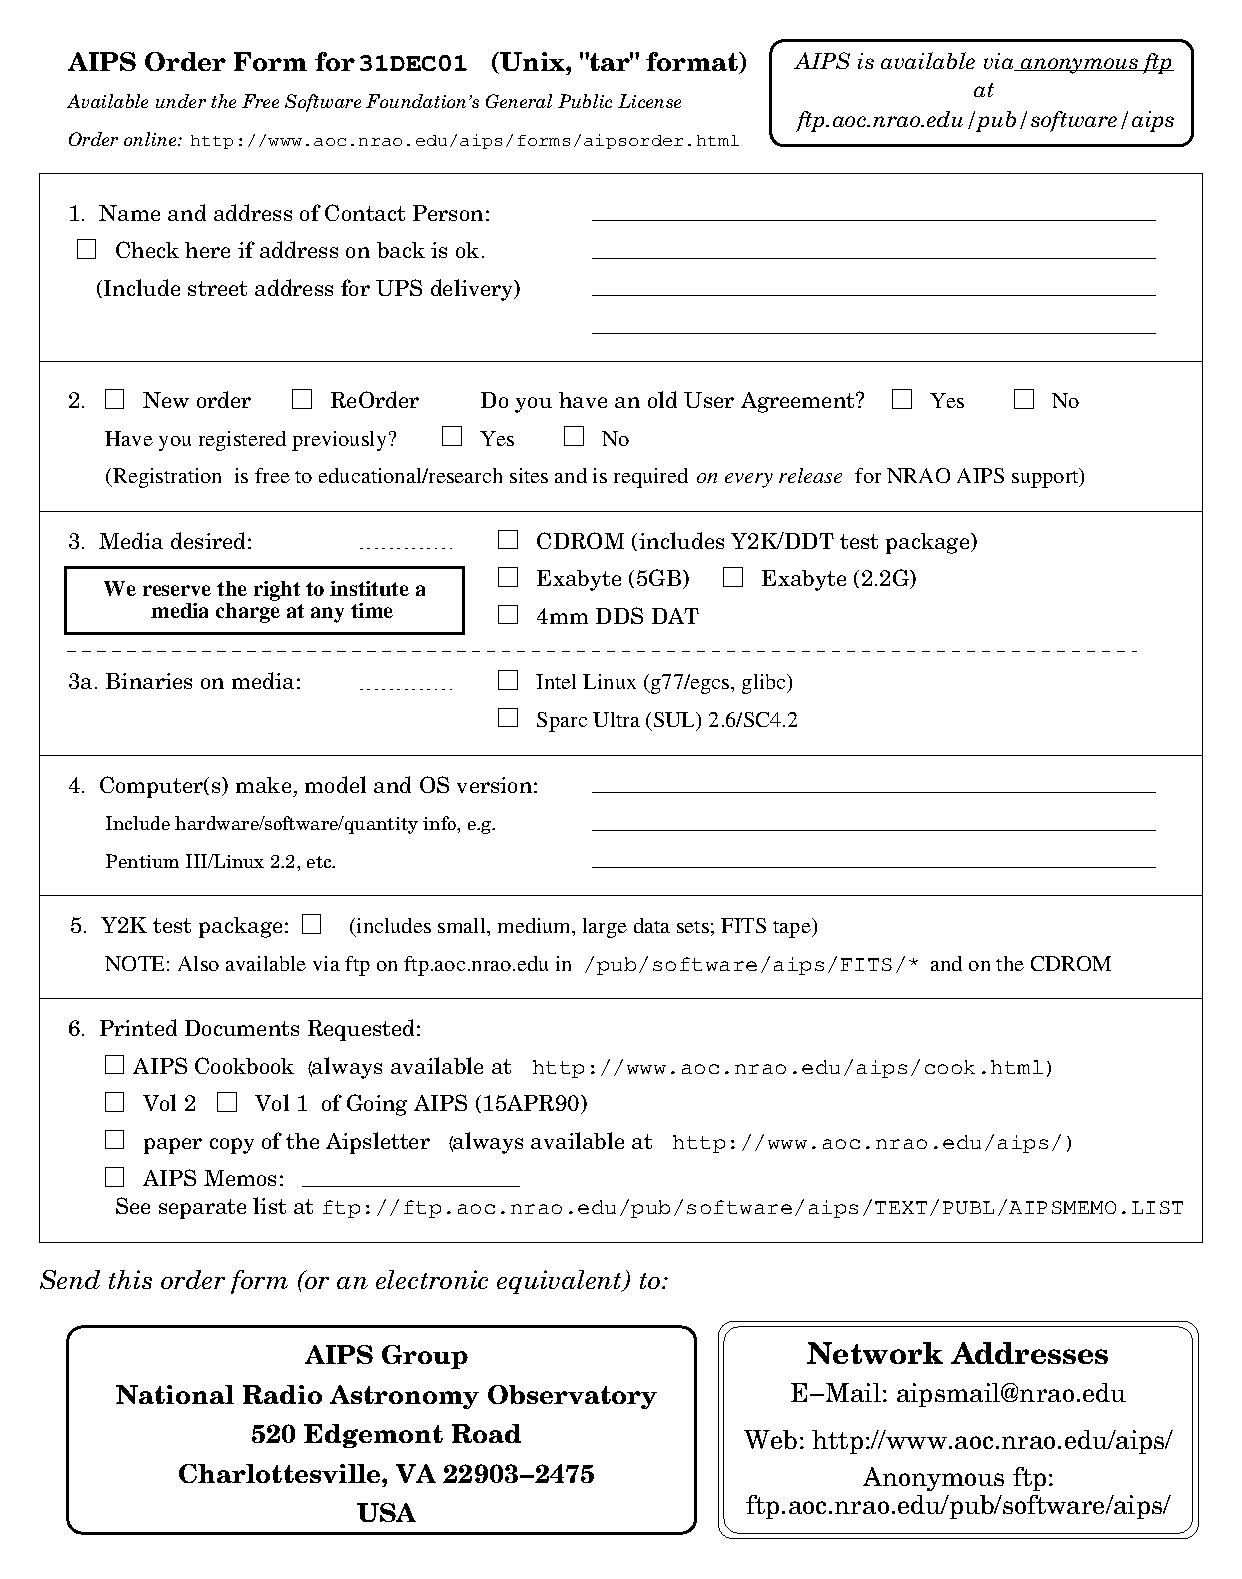
\includegraphics{FIG/AIPSORDER.PS}}}
%\vfill\eject
\vbox to 4.4in{
\vspace{12pt}
%\centerline{\rotatebox{-90}{\resizebox{!}{3.5in}{%
%\includegraphics{FIG/Mandrill.color.plt}}}}
\centerline{\resizebox{!}{3.5in}{\includegraphics{FIG/Mandrill.eps}}}
\vspace{12pt}
\centerline{{\huge \tt \AIPRELEASE}}
\vspace{12pt}
\vfill}
\phantom{...}
\centerline{\resizebox{!}{!}{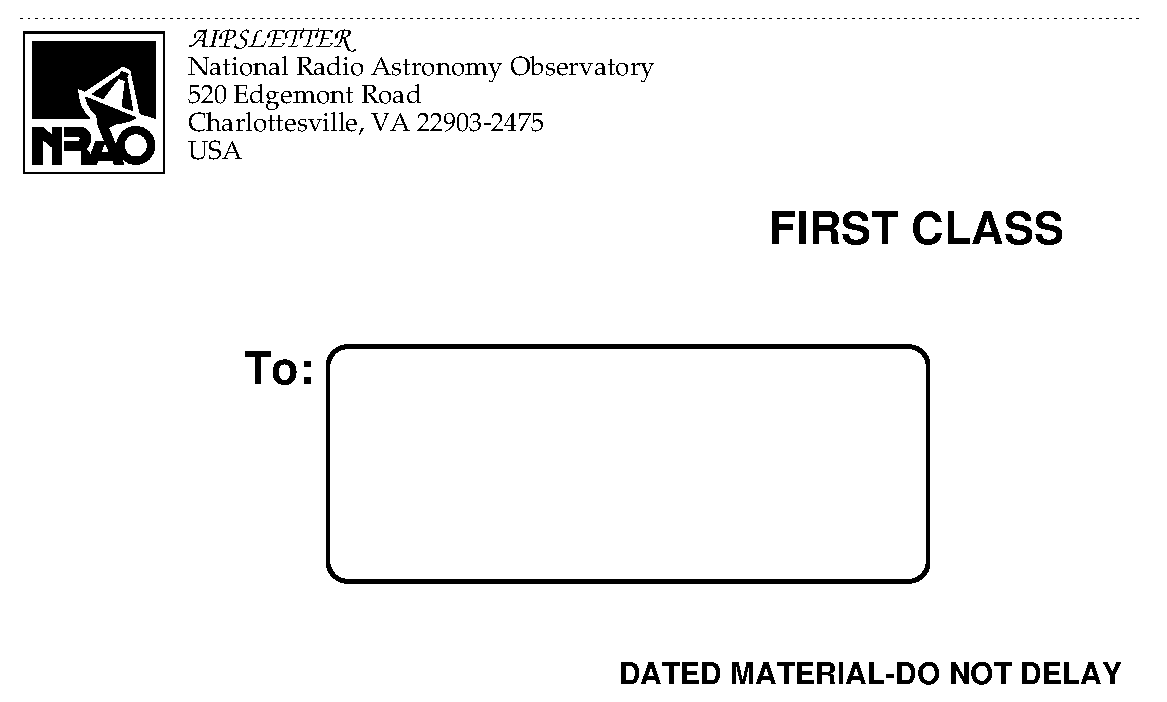
\includegraphics{FIG/AIPSLETM.PS}}}

\end{document}
